\section{Otro tipo de asignación}

\begin{frame}{Definición}
    Otra forma de escoger un estado microscópico compatible es tomando un promedio.
    \begin{columns}
        \begin{column}{0.5\textwidth}
            Un promedio sobre el conjunto
            \begin{equation}
                \Omega_{\mcC}(\rho_{\ef}) = \{\ket{\psi}\in\hilbert_{m}:\, \mcC(\dyad{\psi}) = \rho_{\ef}  \}.\nonumber
            \end{equation}
            La aplicación de asignación promedio es el promedio sobre dicho conjunto, \ie 
            \begin{equation}
            \mcA_{\mcC}^{\avg}(\rho_{\ef}) =\int d \mu\,\, \delta(\mcC(\dyad{\psi})-\rho_{\ef})\,\dyad{\psi}.
            \end{equation}
        \end{column}
        \begin{column}{0.5\textwidth}
            La solución analítica a la ecuación (\ref{eq:AvgMap}) es complicada, pero ha sido encontrada por los doctores C. Pineda y R. Uriostegui del Instituto de Física de la UNAM, para el caso en que la aplicación de grano grueso va de $\densityspace{4}$ a $\densityspace{2}$. Esto es, del espacio de dos partículas de dos niveles, al espacio de una partícula de dos niveles. Aquí no se profundizará en dicho resultado, pero se utilizará para poder comparar ambas aplicaciones de asignación.
        \end{column}
    \end{columns}
\end{frame}

\begin{frame}{Diferencia}
    Nos preguntamos sobre la diferencia entre el estado de máxima entropía y el estado promedio, como una función del parámetro $p_{1}$ ie{} 
    \begin{equation}
        \text{d}_{F}\qty(\avgass(\rho_{\ef}),\maxass(\rho_{\ef}))(p_{1},r_{\ef}).\nonumber
    \end{equation}
\end{frame}

\begin{frame}{Diferencia}
    \begin{figure}
        \centering
        \begin{subfigure}{.45\textwidth}
          \centering
          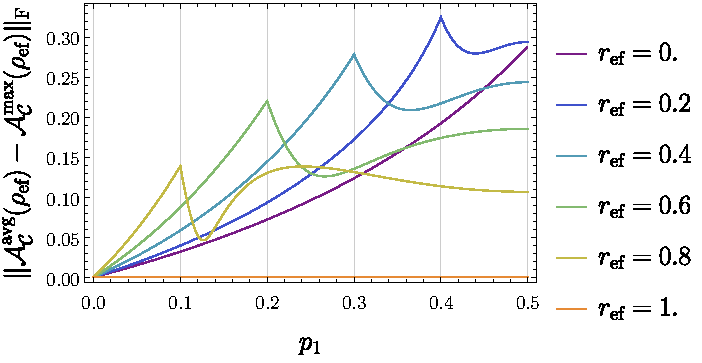
\includegraphics[width=1.\linewidth]{figures/avg_results/dist_maxent_avg_vs_p.pdf}
        \end{subfigure}%
        \begin{subfigure}{.45\textwidth}
          \centering
          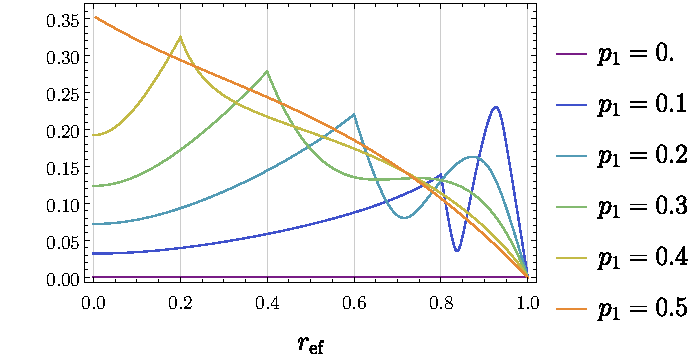
\includegraphics[width=1.\linewidth]{figures/avg_results/dist_maxent_avg_vs_z.pdf}
        \end{subfigure}
        \caption{Distancia de Frobenius entre asignaciones como función de $p_{1}$ para diferentes valores de $r_{z}$, y como función de $r_{z}$ para diferentes valores de $p_{1}$.}
    \end{figure}
\end{frame}

\begin{frame}{Diferencia}
    \begin{figure}[ht!]
        \centering
        \begin{subfigure}{.45\textwidth}
          \centering
          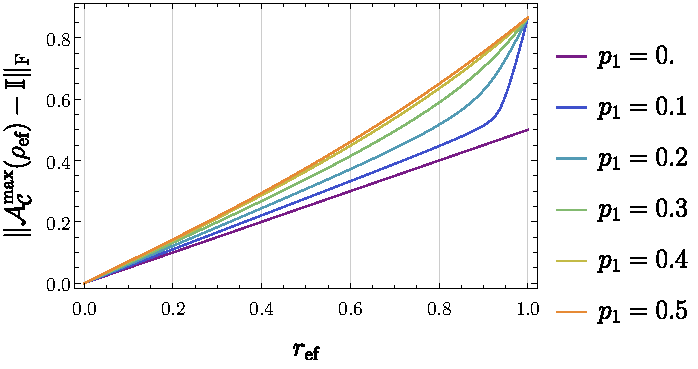
\includegraphics[width=1.\linewidth]{figures/avg_results/dist_maxent_or_vs_p.pdf}
        \end{subfigure}%
        \begin{subfigure}{.45\textwidth}
          \centering
          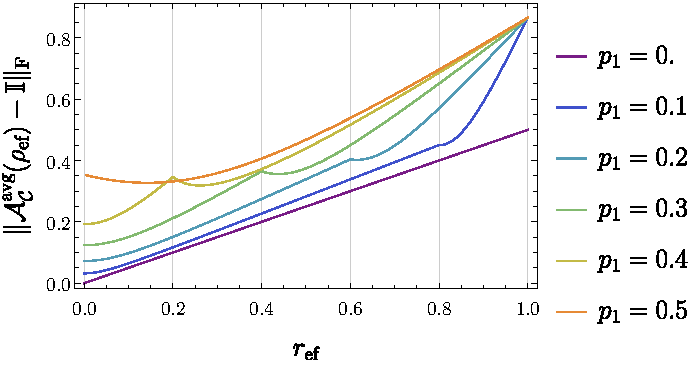
\includegraphics[width=1.\linewidth]{figures/avg_results/dist_avg_or_vs_p.pdf}
        \end{subfigure}
        \caption{Distancia entre asignaciones y el estado máximamente mezclado.}
    \end{figure}
\end{frame}

\begin{frame}{Diferencia}
    \begin{itemize}
        \item Iguales si el estado efectivo inicial es puro y si la aplicación de grano grueso se reduce a una traza parcial ($p_{1}\in\{0,1\}$).
        \item Por otro lado, mientras que la asignación de máxima entropía asigna al estado máximamente mezclado $\Id_{2}/2$ el estado máximamente mezclado correspondiente, $\Id_{4}/4$, la asignación promedio no hace esto.
    \end{itemize}
    \begin{center}
        El estado efectivo evolucionado es $(\mcC\circ\mcE_{t}\circ\mcA_{\mcC})(\rho_{\ef}(0))$.
        \begin{equation}
            mcA_{\mcC}^{\max}(\rho_{\ef}(0))=\mcA_{\mcC}^{\avg}(\rho_{\ef}(0)) \qquad \Rightarrow \qquad \Gamma_{t}^{\avg}=\Gamma_{t}^{\max} \nonumber
        \end{equation}
    \end{center}
\end{frame}

\begin{frame}{Dinámicas separables}
    \lipsum[1]
\end{frame}

\begin{frame}{Dinámicas separables}
    \begin{figure}[ht!]
        \centering
        \begin{subfigure}{0.5\textwidth}
          \centering
          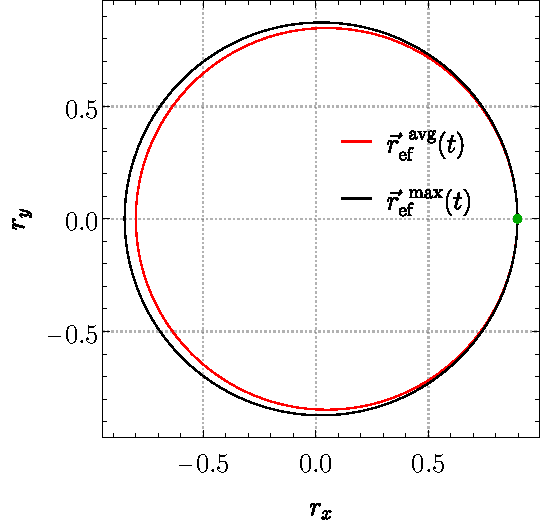
\includegraphics[width=0.8\linewidth]{figures/avg_results/local_AvgVSMax_p2=0.1_r=0.9_w1=0_w2=1.pdf}
          \caption{$H=\Id\otimes\pauli{3}$}
        \end{subfigure}%
        \begin{subfigure}{0.5\textwidth}
          \centering
          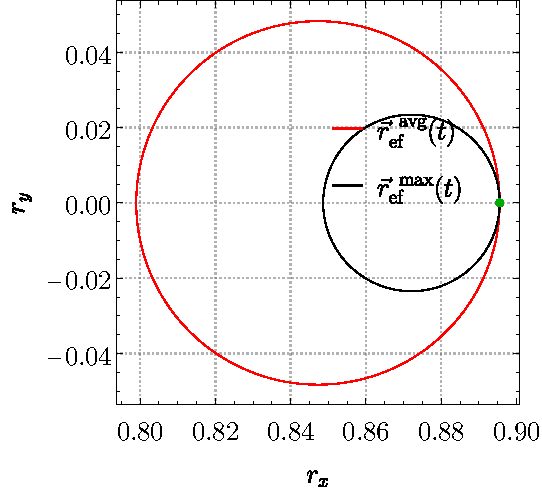
\includegraphics[width=0.8\linewidth]{figures/avg_results/local_AvgVSMax_p2=0.1_r=0.9_w1=1_w2=0.pdf}
          \caption{$H=\pauli{3}\otimes\Id$}
        \end{subfigure}
        \caption{Variaciones correspondientes a la dinámica efectiva inducida por diferentes hamiltonianos en un sistema de dos partículas partiendo de un estado efectivo inicial (verde) tal que $r_{\ef}=0.9$ y $r_{z}\approx0.09$. En rojo, la evolución del estado promedio. En negro, la del estado de máxima entropía. \label{ap:EffDunAVGvsMaxEnt1}}
    \end{figure}
\end{frame}

\begin{frame}{Dinámicas separables}
    \begin{figure}[ht!]
        \centering
        \begin{subfigure}{0.5\textwidth}
          \centering
          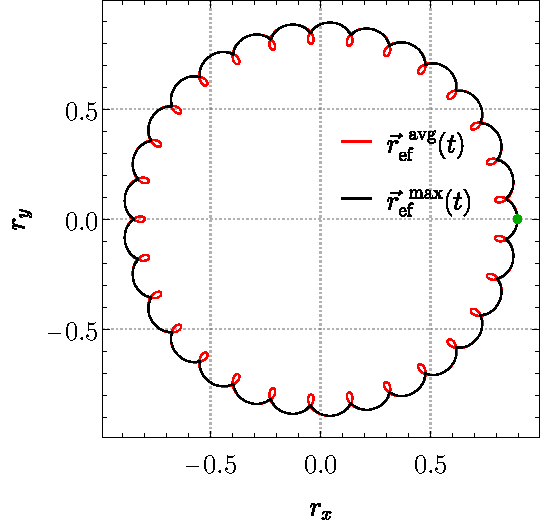
\includegraphics[width=0.8\linewidth]{figures/avg_results/local_AvgVSMax_p2=0.1_r=0.9_w1=30_w2=1.pdf}
          \caption{$H=30\pauli{3,1}+\pauli{3}$}
        \end{subfigure}%
        \begin{subfigure}{0.5\textwidth}
          \centering
          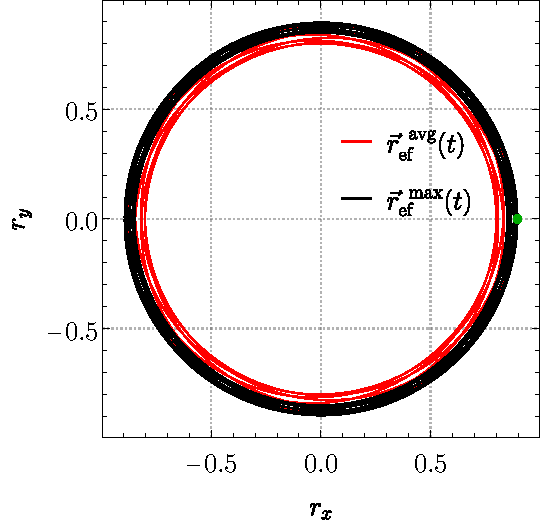
\includegraphics[width=0.8\linewidth]{figures/avg_results/local_AvgVSMax_p2=0.1_r=0.9_w1=1_w2=10.pdf}
          \caption{$H=\pauli{3,1}+10\pauli{3}$}
        \end{subfigure}
        \caption{Variaciones correspondientes a la dinámica efectiva inducida por diferentes hamiltonianos en un sistema de dos partículas partiendo de un estado efectivo inicial (verde) tal que $r_{\ef}=0.9$ y $r_{z}\approx0.09$. En rojo, la evolución del estado promedio. En negro, la del estado de máxima entropía. \label{ap:EffDunAVGvsMaxEnt2}}
    \end{figure}
\end{frame}

\begin{frame}{Compuerta SWAP}
    \lipsum[1]
\end{frame}

\begin{frame}{Discusión}
    La aplicación de asignación promedio no es fácilmente escalable a sistemas de $n$ qudits. Por otro lado, como se mostró en la sección \ref{sec:maxentcons}, utilizar el Principio de Máxima Entropía permite dichas extensiones de forma directa. Esto abre un camino directo a la obtención de resultados analíticos, cosa que se ha aprovechado. 
    
    En caso de no haber una razón para incluir únicamente estados puros en la definición de la aplicación de asignación promedio, esta restricción es tan arbitraria como considerar que todos los estados microscópicos compatibles con el estado efectivo son igualmente probables (suposición que también se hace). La elección de los estados a considerar, así como la medida sobre la que realizar la integración, son elementos de información que inyectan un sesgo a los resultados que puedan ser obtenibles. La aplicación de asignación de máxima entropía utiliza únicamente la información accesible al observador, y puede ser modificado para incluir nuevas restricciones. 
\end{frame}